% --------------------------------------------------------------------------------------------------
% Section: Dataset
% --------------------------------------------------------------------------------------------------

\section{Dataset}

% Overview of the dataset section: describes data source, annotation, preprocessing, and limitations
% Includes dataset origin, organization, formats, class distribution, augmentation, and challenges

% --------------------------------------------------------------------------------------------------
% Subsection: Data Source
% --------------------------------------------------------------------------------------------------

\subsection{Data Source}

% Specifies the origin and name of the dataset used, including its full name and public availability
The dataset used in this project is the {\textit{IQ-OTH/NCCD - Lung Cancer Dataset}} (The Iraq-Oncol
ogy Teaching Hospital/National Center for Cancer Diseases), publicly available from The Cancer 
Imaging Archive (TCIA). \cite{subhajeet_das_2025}

% Describes collection time frame, institutions involved, and nature of the data (CT scans)
This dataset was collected in the above-mentioned specialist hospitals over a period of three months 
in fall 2019. It includes CT scans (originally collected in DICOM format) of patients diagnosed 
with lung cancer in different stages, as well as healthy subjects. 

% Details image structure and patient demographics for clinical diversity
Each scan contains several slices (from 80 to 200), each of them represents an image of the human 
chest with different sides and angles. The cases vary in gender, age, educational attainment, area 
of residence, and living status. Some of them are employees of the Iraqi ministries of Transport and 
Oil, others are farmers and gainers. Most of them come from places in the middle region of Iraq,  
particularly, the provinces of Baghdad, Wasit, Diyala, Salahuddin, and Babylon.

\vspace{1em}
\begin{center} 
    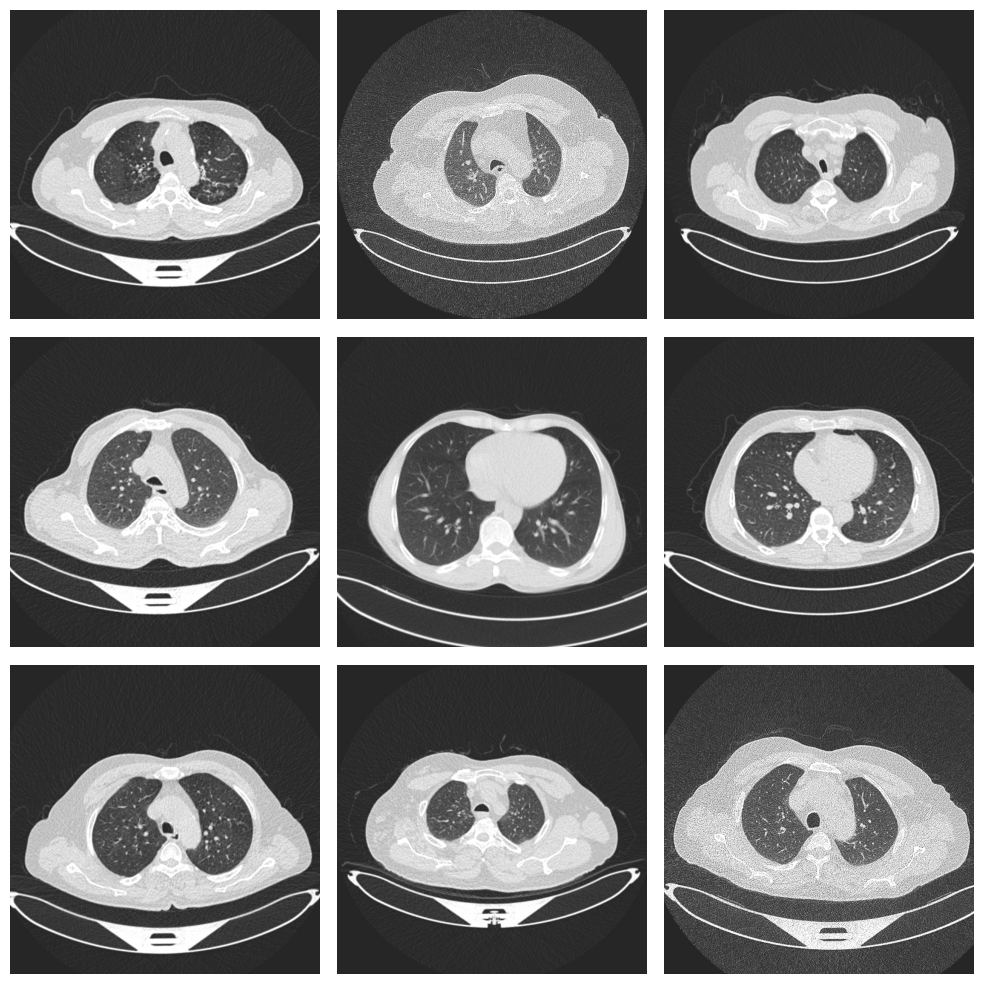
\includegraphics[width=0.7\textwidth]{../assets/02-dataset/ct-scans.png} 

    \small\textit{Figure 1. CT scan samples from dataset.}
\end{center}
\vspace{1em}

% --------------------------------------------------------------------------------------------------
% Subsection: Data Description
% --------------------------------------------------------------------------------------------------

\subsection{Data Description: Properties, Types and Formats}

% Number of images, number of patients, format, and image resolution properties
The IQ-OTH/NCCD lung cancer dataset consists of 3.609 chest CT scan images collected from 110 
individual patients. Each image is stored in JPEG format with non-uniform resolutions. 

% Figure: distribution of image sizes in the dataset
\vspace{1em}
\begin{center} 
    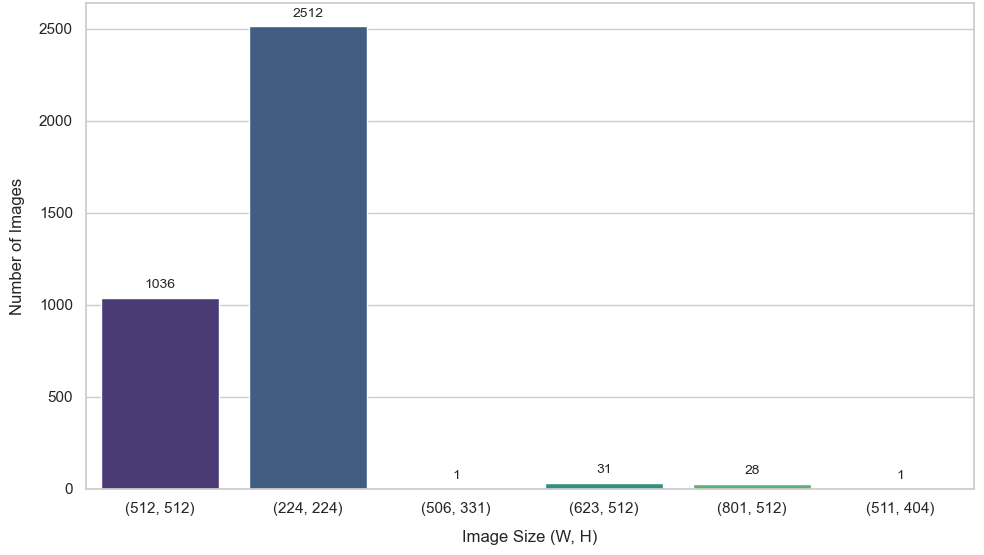
\includegraphics[width=\textwidth]{../assets/02-dataset/image-size-distribution.png}
    \small\textit{Figure 2. Distribution of images size.}
\end{center}
\vspace{1em}

% --------------------------------------------------------------------------------------------------
% Subsection: Data Annotation
% --------------------------------------------------------------------------------------------------

\subsection{Data Annotation: Methods and Categories}

% Classification categories and folder-based organization
The dataset was manually organized into three distinct folders, each corresponding to a diagnostic 
category used for classification:
\begin{itemize}
    \item \textbf{Normal} – images without visible nodules or abnormalities
    \item \textbf{Benign} – images containing nodules classified as non-cancerous
    \item \textbf{Malignant} – images containing nodules classified as cancerous
\end{itemize}  

% Description of labeling process and annotator expertise
The labeling of each image was performed by a team of experienced oncologists and radiologists, 
ensuring a high degree of clinical accuracy and reliability in the annotation process. This 
expert-labeled dataset forms a strong foundation for training a supervised learning model in a 
sensitive medical context.

% Explains how image folders map to supervised classification model training
This folder-based organization enabled the model to correctly associate each image with its 
corresponding class label during training and evaluation. The distribution of these labeled samples 
is presented in \hyperlink{figura3}Figure 3.

% --------------------------------------------------------------------------------------------------
% Subsection: Data Preprocessing
% --------------------------------------------------------------------------------------------------

\subsection{Data Preprocessing: Augumentation and Cleaning}

% Rationale for discarding non-square images and resizing; importance of uniform input for CNNs
As part of the preprocessing pipeline, non-square images were removed from the dataset prior to 
training. This decision was made to avoid potential issues associated with direct resizing or 
aspect-ratio-preserving padding, both of which can negatively impact the performance of CNN. To 
ensure consistency and compatibility with the input requirements of CNN, all remaining images were 
resized to a uniform resolution of 224×224 pixels. 

% Avoiding padding to reduce irrelevant edge artifacts learned by early convolutional layers
Although techniques such as padding can preserve the original aspect ratio, they introduce 
artificial borders and non-informative regions into the image. These artifacts may be misinterpreted 
by the CNN as meaningful features, especially in the early convolutional layers, which are  
sensitive to spatial patterns. As a result, the model might learn irrelevant cues and generalize  
poorly, particularly in medical imaging tasks where precision is critical.

% Risks of geometric distortion due to naive resizing methods
Furthermore, direct resizing of non-square images to a fixed square input size results in geometric 
distortion, altering the shape, size, and orientation of key anatomical structures such as lung 
nodules. This deformation can obscure clinically relevant patterns and lead to degraded model 
performance, especially in tasks involving subtle morphological differences between classes.

% Figure: image label distribution after preprocessing
\vspace{1em}
\begin{center} 
    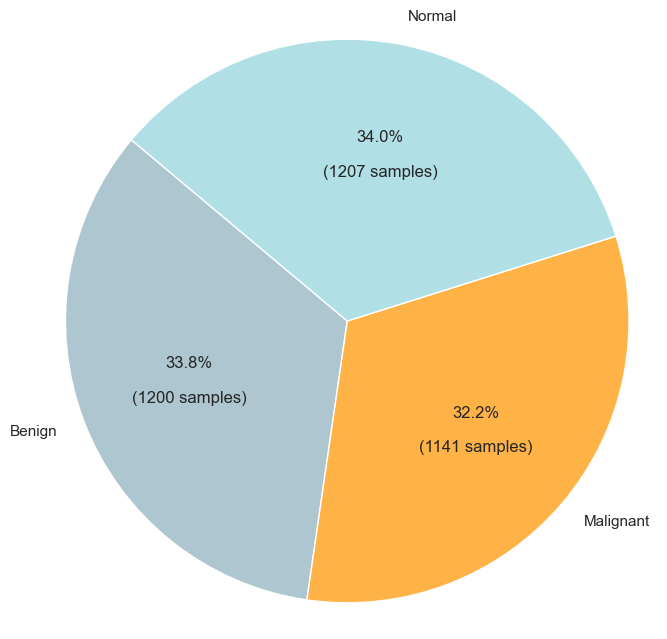
\includegraphics
    [width=0.7\textwidth]{../assets/02-dataset/label-distribution-after-preprocessing.png}
    
    \small\textit{\hypertarget{figura3}Figure 3. Distribution of images label after preprocessing.}
\end{center}
\vspace{1em}

% Description of original class imbalance and justification for augmentation
The original dataset exhibited a significant imbalance among the diagnostic categories, which could 
adversely affect model training and lead to biased predictions. Specifically, the initial dataset 
included: 40 malignant cases, 15 benign cases and 55 normal (non-nodule) cases. To address this 
issue and ensure a more balanced distribution of classes, extensive data augmentation techniques to 
artificially expand the dataset were applied. The goal was to create a more uniform class 
distribution and enhance the model’s ability to generalize across all categories.

% Lists all augmentation methods used to increase class diversity
The augmentation techniques applied include: Horizontal Flip, Vertical Flip, Rotation, Colorjitter, 
Contour Crop, Gaussian Blur, Sharpeness, Contrast and Histogram Equalization 
\cite{subhajeet_das_2025}.

% Figure: comparison of original vs post-augmentation label distribution
\vspace{1em}
\begin{center} 
    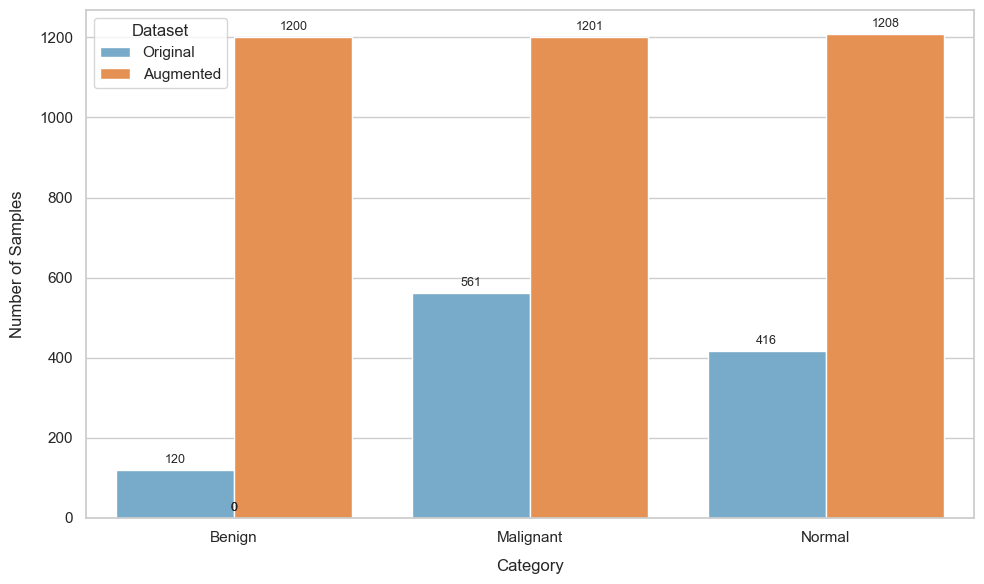
\includegraphics[width=\textwidth]{../assets/02-dataset/label-distribution.png}
    \small\textit{\hypertarget{figura3}Figure 3. Distribution of images label compared to the 
    original dataset.}
\end{center}
\vspace{1em}

% --------------------------------------------------------------------------------------------------
% Subsection: Data Splitting
% --------------------------------------------------------------------------------------------------

\subsection{Data Splitting: Training, Test and Validation}

% Describes data split proportions used for training, validation, and testing
To ensure effective training, evaluation, and generalization of the Convolutional Neural Network 
(CNN), the dataset was split into three subsets using the following proportions: 75\% Training Set, 
15\% Validation Set and 15\% Test Set.

\begin{itemize}
    % Role of training set in feature learning, especially important in complex medical data
    \item \textbf{Effective Learning:} Allocating the majority of the data to the training set 
    ensures that the model has sufficient samples to learn patterns, especially in a medical imaging 
    context where inter-class variations may be subtle and complex.

    % Use of validation set for monitoring training and tuning hyperparameters
    \item \textbf{Hyperparameter Tuning:} The validation set is used to monitor the model’s 
    performance during training and to fine-tune hyperparameters. This helps prevent overfitting by 
    evaluating how well the model generalizes to unseen data during the training process.

    % Independent test set for final model evaluation
    \item \textbf{Unbiased Performance Evaluation:} The test set is strictly separated from the 
    training and validation processes. It provides an objective estimate of the model’s real-world 
    performance, helping ensure that performance metrics are not inflated by exposure to the 
    training data.
\end{itemize}

% Final remark on the importance of proper data partitioning
This division plays a crucial role in the training workflow and contributes to the development of a 
robust and unbiased model.

% --------------------------------------------------------------------------------------------------
% Subsection: Challenges and Limitations
% --------------------------------------------------------------------------------------------------

\subsection{Challenges and Limitations}

% Discusses the primary limitations and potential bottlenecks of the dataset and its impact on model
Despite its usefulness, the IQ-OTH/NCCD dataset presents several limitations:

\begin{itemize}
    % Dataset size limitation and risks of overfitting
    \item \textbf{Limited Dataset Size}: Only 3,609 CT images from 110 patients — a relatively
    small dataset — may lead to overfitting and reduced generalization.

    % Initial class imbalance, especially for benign cases
    \item \textbf{Class Imbalance}: A severe initial imbalance, especially in benign cases, may 
    affect model reliability, despite augmentation efforts.

    % Subjectivity and potential inconsistency in manual labeling
    \item \textbf{Annotation Variability}: Expert annotations can still be subjective, with 
    interobserver variability potentially introducing label noise.

    % Use of 2D slices omits volumetric (3D) diagnostic context
    \item \textbf{Lack of 3D Context}: Working with individual 2D slices disregards spatial 
    continuity across scans, possibly omitting valuable diagnostic information.

    % JPEG compression and quality variance may impact feature extraction
    \item \textbf{Resolution Inconsistency}: JPEG compression artifacts and varying image quality
    hinder feature consistency and model accuracy.

    % Trade-offs made in preprocessing may sacrifice valuable data
    \item \textbf{Preprocessing Trade-offs}: Removal of non-square images and resizing may discard
    informative content or distort lesion morphology.

    % Dataset demography restricts model generalization across populations
    \item \textbf{Geographic and Demographic Bias}: Patients from a specific region in Iraq limit 
    generalizability across different populations and scanner environments.
\end{itemize}
